\documentclass[
  bibliography=totoc,     % Literatur im Inhaltsverzeichnis
  captions=tableheading,  % Tabellenüberschriften
  titlepage=firstiscover, % Titelseite ist Deckblatt
]{scrartcl}

% Paket float verbessern
\usepackage{scrhack}

% Warnung, falls nochmal kompiliert werden muss
\usepackage[aux]{rerunfilecheck}

% unverzichtbare Mathe-Befehle
\usepackage{amsmath}
% viele Mathe-Symbole
\usepackage{amssymb}
% Erweiterungen für amsmath
\usepackage{mathtools}

% Fonteinstellungen
\usepackage{fontspec}
% Latin Modern Fonts werden automatisch geladen
% Alternativ:
%\setromanfont{Libertinus Serif}
%\setsansfont{Libertinus Sans}
%\setmonofont{Libertinus Mono}
\recalctypearea % Wenn man andere Schriftarten gesetzt hat,
% sollte man das Seiten-Layout neu berechnen lassen

% deutsche Spracheinstellungen
\usepackage{polyglossia}
\setmainlanguage{german}


\usepackage[
  math-style=ISO,    % ┐
  bold-style=ISO,    % │
  sans-style=italic, % │ ISO-Standard folgen
  nabla=upright,     % │
  partial=upright,   % ┘
  warnings-off={           % ┐
    mathtools-colon,       % │ unnötige Warnungen ausschalten
    mathtools-overbracket, % │
},                       % ┘
]{unicode-math}

% traditionelle Fonts für Mathematik
\setmathfont{Latin Modern Math}
% Alternativ:
%\setmathfont{Libertinus Math}

\setmathfont{XITS Math}[range={scr, bfscr}]
\setmathfont{XITS Math}[range={cal, bfcal}, StylisticSet=1]

% Zahlen und Einheiten
\usepackage[
locale=DE,                   % deutsche Einstellungen
separate-uncertainty=true,   % immer Fehler mit \pm
per-mode=symbol-or-fraction, % / in inline math, fraction in display math
]{siunitx}

% chemische Formeln
\usepackage[
version=4,
math-greek=default, % ┐ mit unicode-math zusammenarbeiten
text-greek=default, % ┘
]{mhchem}

% richtige Anführungszeichen
\usepackage[autostyle]{csquotes}

% schöne Brüche im Text
\usepackage{xfrac}

% Standardplatzierung für Floats einstellen
\usepackage{float}
\floatplacement{figure}{htbp}
\floatplacement{table}{htbp}

% Floats innerhalb einer Section halten
\usepackage[
section, % Floats innerhalb der Section halten
below,   % unterhalb der Section aber auf der selben Seite ist ok
]{placeins}

% Seite drehen für breite Tabellen: landscape Umgebung
\usepackage{pdflscape}

% Captions schöner machen.
\usepackage[
  labelfont=bf,        % Tabelle x: Abbildung y: ist jetzt fett
  font=small,          % Schrift etwas kleiner als Dokument
  width=0.9\textwidth, % maximale Breite einer Caption schmaler
]{caption}
% subfigure, subtable, subref
\usepackage{subcaption}

% Grafiken können eingebunden werden
\usepackage{graphicx}
% größere Variation von Dateinamen möglich
\usepackage{grffile}

% schöne Tabellen
\usepackage{booktabs}

% Verbesserungen am Schriftbild
\usepackage{microtype}

% Literaturverzeichnis
\usepackage[style=alphabetic,]{biblatex}
% Quellendatenbank
\addbibresource{lit.bib}
\addbibresource{programme.bib}

% Hyperlinks im Dokument
\usepackage[
  unicode,        % Unicode in PDF-Attributen erlauben
  pdfusetitle,    % Titel, Autoren und Datum als PDF-Attribute
  pdfcreator={},  % ┐ PDF-Attribute säubern
  pdfproducer={}, % ┘
]{hyperref}
% erweiterte Bookmarks im PDF
\usepackage{bookmark}

% Trennung von Wörtern mit Strichen
\usepackage[shortcuts]{extdash}

\title{V21: Optisches Pumpen}
\author{
  Simon Schulte
  \texorpdfstring{
    \\
    \href{mailto:simon.schulte@udo.edu}{simon.schulte@udo.edu}
  }{}
  \texorpdfstring{\and}{, }
  Tim Sedlaczek
  \texorpdfstring{
    \\
    \href{mailto:tim.sedlaczek@udo.edu}{tim.sedlaczek@udo.edu}
  }{}
}
\publishers{TU Dortmund – Fakultät Physik}

\date{Durchführung: 09.05.2018\\
      Abgabe: 16.05.2018}


\begin{document}

\maketitle
\thispagestyle{empty}
\setcounter{page}{1}
\pagenumbering{arabic}
\section{Theorie}
\label{sec:theorie}
Ziel des Versuchs ist die Untersuchung von Übergängen bestimmter
Energieniveaus in Rubidium-Isotopen. Daraus lassen sich die Lande-Faktoren,
der Kernspin der Isotope und die Größe der Zeeman-Aufspaltung berechnen. \\
In allen Atomen befinden sich Elektronen auf sogenannten Schalen um den
Atomkern. Auf diesen Schalen besitzen sie feste Energien, zwischen welchen
allerdings Übergänge stattfinden können. Dazu muss Energie, die exakt der
Differenz der Niveaus entspricht von den Elektronen abgegeben oder aufgenommen
werden. Dies geschieht über die Aufnahme oder Abgabe von Photonen der
passenden Frequenz. Die äußeren Niveaus, also jene mit den größten Energien,
sind dabei je nach Temperatur unterschiedlich besetzt. Die Besetzungszahl eines
Niveaus folgt dabei einer Boltzmann Verteilung, sodass für das Verhältnis der
Besetzungszahlen zweier Niveaus gilt:
%
\begin{equation}
  \frac{N_2}{N_1}=\frac{g_2}{g_1}\frac{\exp\left(-\sfrac{W_2}{\symup{k_B}T}\right)}{\exp(-\sfrac{W_1}{\symup{k_B}T})}
\end{equation}
%
Hierbei beschreiben die $W_i$ die Energien der Zustände, die $g_{\symup{i}}$ die
Lande-Faktoren, welche beschreiben, wie viele Zustände zu der entsprechenden
Energie gehören, sowie $\symup{k_B}$ die Boltzmann-Konstante und $T$ die
Temperatur. \\
Mit Hilfe des optischen Pumpens kann eine Abweichung von dieser Verteilung
erzeugt werden. Diese kann soweit gehen, dass eine Besetzungsinversion
entsteht. Eine so entstehende nicht-thermische Verteilung ermöglicht es,
einzelne Übergänge zu induzieren, sodass Photonen dieser Energie überwiegend
das Spektrum prägen. Über die Vermessung dieses Lichtes lässt sich der
Energieabstand $\symup{h}\nu=W_2-W_1$ der Niveaus messen.

\subsection{Energieniveaus der Elektronen eines Atomes}
%
Die Verteilung der Elektronen auf verschiedene Energieniveaus innerhalb des
Atomes folgt aus Auswahlregeln verschiedener Quantenzahlen. Aus dem
Gesamtdrehimpuls $\vec{\mathup{J}}$ der Elektronenhülle folgt ein magnetisches Moment
$\vec{\mu}_\mathup{J}=-g_{\symup{J}}\mu_{\symup{B}}\vec{\mathup{J}}$. Der Faktor $g_{\symup{J}}$
berücksichtigt dabei, dass das Gesamtmoment aus Spin $\mathup{S}$ und Drehimpuls $\mathup{L}$
folgt. Es gilt
%
\begin{align*}
  |\vec{\mu}_\mathup{J}|=&g_{\symup{J}}\mu_{\symup{B}}\sqrt{\mathup{J}(\mathup{J}+1)},\;\text{wobei} \\
  |\vec{\mu}_\mathup{L}|=&-\mu_{\symup{B}}\sqrt{\mathup{L}(\mathup{L}+1)}\;\text{und} \\
  |\vec{\mu}_\mathup{S}|=&-g_{\symup{S}}\mu_{\symup{B}}\sqrt{\mathup{S}(\mathup{S}+1)}\;.
\end{align*}
%
Das Gesamtdrehmoment $\vec{\mu}_\mathup{J}$ der Elektronenhülle präzediert dabei um den
Gesamtdrehimpuls $\vec{\mathup{J}}$. Daher trägt stets nur der parallele Anteil dieses
Drehimpulses zum magnetischen Moment bei. $g_{\symup{J}}$ ist also abhängig von
$\mathup{J}$, $\mathup{S}$ und $\mathup{L}$. Es ergibt sich
%
\begin{equation}
  g_{\symup{J}}=\frac{\num{3.0023}\mathup{J}(\mathup{J}+1)+\num{1.0023}\left(\mathup{S}(\mathup{S}+1)-\mathup{L}(\mathup{L}+1)\right)}{2\mathup{J}(\mathup{J}+1)}
  \label{eq:gj}
\end{equation}
%
Wird ein äußeres Magnetfeld angelegt, so spaltet sich das
Spektrum weiter auf. Es gilt
%
\begin{equation}
  U_\text{mag}=-\vec{\mu}_\mathup{J}\cdot\vec{B}
\end{equation}
%
Hieraus folgt eine Richtungsquantelung der Energie:
%
\begin{equation}
  U_\text{mag}=g_{\symup{J}}\mu_{\symup{B}}B\cdot M_\mathup{J},\quad M_\mathup{J}\in[-\mathup{J},\mathup{J}]
\end{equation}
%
Bei Anlegen eines äußeren Magnetfeldes wird also über den Zeeman-Effekt jedes
Energieniveau in $2\mathup{J}+1$ Unterniveaus aufgespalten. Die Anzahl der so
entstehenden Niveaus ist abhängig von dem sich aus Gesamtdrehimpuls der
Elektronenhülle $\mathup{J}$ und dem Kernspin $\mathup{I}$ ergebenden Gesamtdrehimpuls $\mathup{F}$ des
Atomes.
%
\begin{figure}[h]
  \centering
  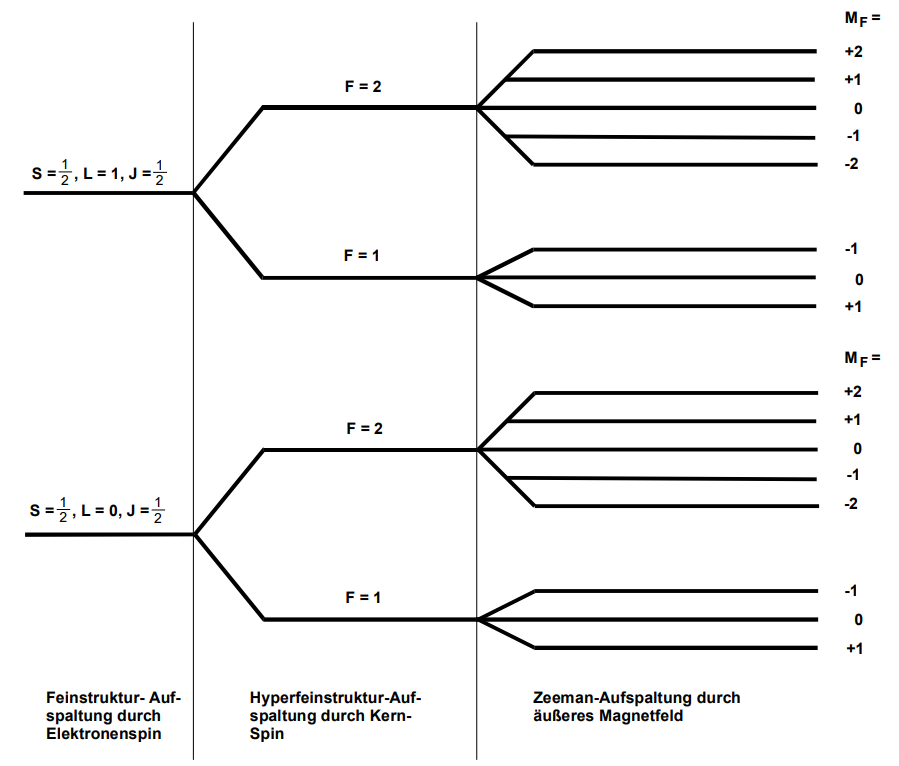
\includegraphics[width=0.75\textwidth]{Aufspaltung.jpg}
  \caption{Aufspaltung der Energieniveaus innerhalb eines Atomes. Dargestellt
  sind die Feinstrukturaufspaltung durch den Elektronenspin, die
  Hyperfeinstrukturaufspaltung durch den Kernspin, sowie die Zeeman-Aufspaltung
  durch ein äußeres Magnetfeld. \cite{anleitung}}
  \label{fig:aufspaltung}
\end{figure}

\subsection{Optisches Pumpen}
%
Die beiden in diesem Versuch betrachteten Rubidium-Isotope haben beide einen
Kernspin $I \neq 0$. Das Verfahren des optischen Pumpens wird anhand eines Beispiel-Systems
betrachtet. Es handelt sich dabei zunächst vereinfacht um ein Alkali-Atom ohne Kernspin $\vec{I}$.
Der Grundzustand ist der Zustand $^2S_{\sfrac{1}{2}}$. Angeregte Zustände sind
$^2P_{\sfrac{1}{2}}$, sowie $^2P_{\sfrac{3}{2}}$.
%
\begin{figure}[htb]
  \centering
  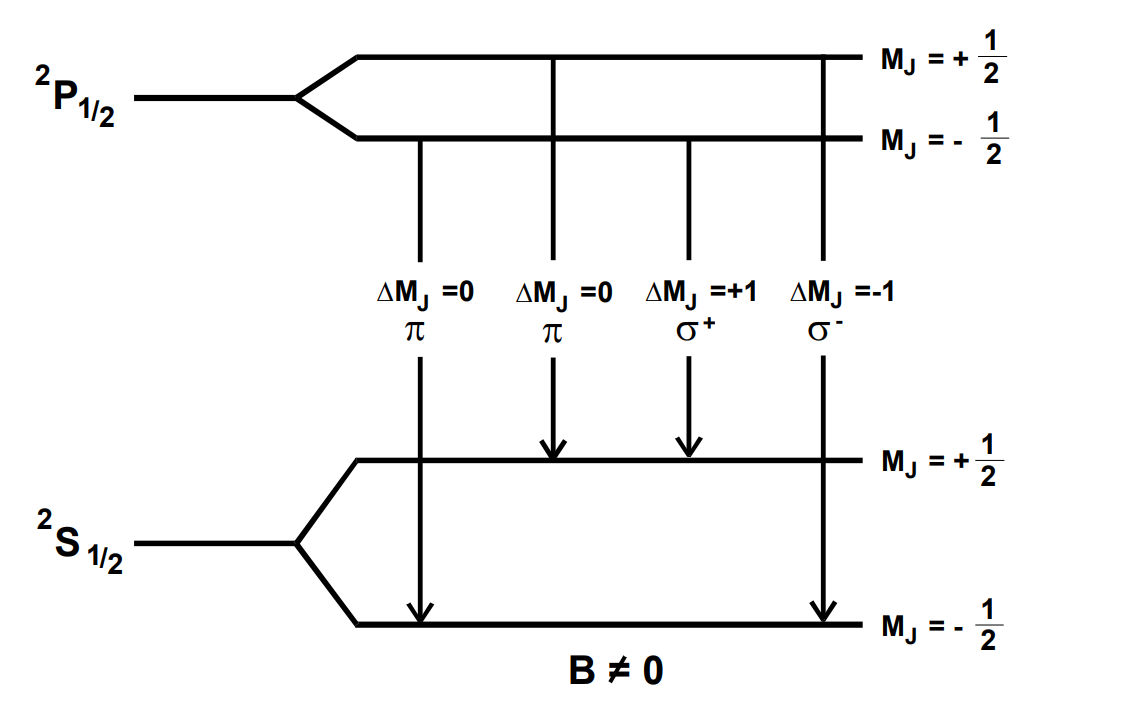
\includegraphics[width=0.9\textwidth]{Beispiel.jpg}
  \caption{Aufspaltung der $S$- und $P$-Niveaus eines Beispiel-Atomes. Rechts:
  Zeeman-Aufspaltung des $^2P_{\sfrac{1}{2}}$- sowie des
  $^2S_{\sfrac{1}{2}}$-Niveaus. \cite{anleitung}}
  \label{fig:beispiel}
\end{figure}
\noindent
Die Energieniveaus, sowie deren Aufspaltung im Magnetfeld sind in
Abbildung~\ref{fig:beispiel} skizziert. Das bei den rechts skizzierten
Übergängen emittierte Licht besitzt spezielle Polarisationseigenschaften. Das
$\sigma^+$-Licht ist rechtszirkular polarisiert (also
$\vec{s}\nparallel\vec{k}$), während das $\sigma^-$-Licht linkszirkular
polarisiert ist (also $\vec{s}\parallel\vec{k}$). Beide Linien erscheinen nur
parallel zum Magnetfeld in dieser Polarisation und sonst linear polarisiert.
Die $\pi$-Linien hingegen sind linear polarisiert und werden nicht parallel zum
Magnetfeld abgestrahlt, da es sich hierbei um Dipolstrahlung handelt.
%
\begin{figure}[htb]
  \centering
  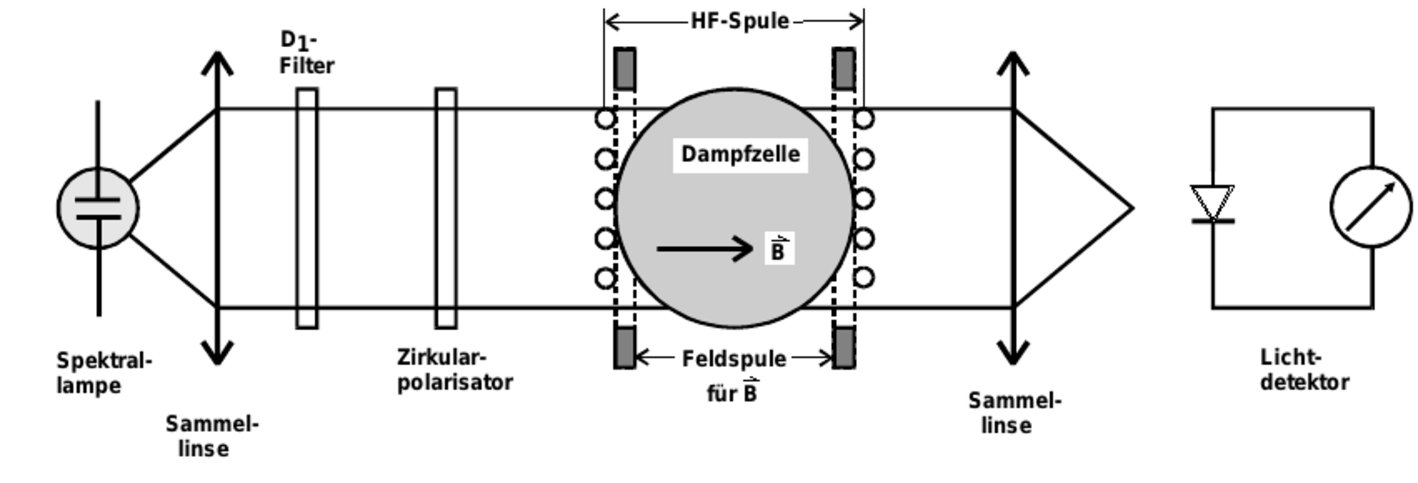
\includegraphics[width=\textwidth]{Versuchsaufbau.pdf}
  \caption{Schematische Darstellung des Versuchsaufbaus \cite{anleitung}.}
  \label{fig:aufbau}
\end{figure}
\noindent
Abbildung~\ref{fig:aufbau} zeigt den schematischen Aufbau der verwendeten
Apparatur. Eine Spektrallampe strahlt Licht in die Apparatur ein. Aus diesem
Licht wird mit Hilfe eines $\text{D}_1$-Filters und eines Polarisationsfilters
rechtszirkular polarisiertes $\text{D}_1$-Licht. Der einzige mögliche
Energieübergang innerhalb der Atome in der Dampfzelle ist derjenige von
$^2\symup{S}_{\sfrac{1}{2}}$ (mit $M_\mathup{J}=-\sfrac{1}{2}$) zu
$^2P_{\sfrac{1}{2}}$ (mit $M_\mathup{J}=+\sfrac{1}{2}$), sowie rückwärts durch
spontane Emission. Beim rückwärtigen Prozess werden allerdings beide
Zeeman-Niveaus des $^2\symup{S}_{\sfrac{1}{2}}$-Niveaus besetzt, sodass im
Laufe der Zeit das Niveau $^2\symup{S}_{\sfrac{1}{2}}$ (mit
$M_\mathup{J}=+\sfrac{1}{2}$) angereichert und das
$^2\symup{S}_{\sfrac{1}{2}}$-Niveau (mit $M_\mathup{J}=-\sfrac{1}{2}$)
\enquote{leergepumpt} wird. Dies hat eine Umkehr der Besetzung im S-Niveau zur
Folge. Experimentell beobachten lässt sich diese Entwicklung über die
Transparenz des Dampfes für Licht.
%
\begin{figure}[htb]
  \centering
  \includegraphics[width=0.6\textwidth]{transparenz.pdf}
  \caption{Verlauf der Transparenz der Dampfzelle in Abhängigkeit der Zeit. Das $M_\mathup{J}=-\sfrac{1}{2}$-Niveau wird \enquote{leergepumpt}\cite{anleitung}.}
  \label{fig:transparenz}
\end{figure}
\noindent
Wird Licht (einer bestimmten Energie) von dem Dampf absorbiert, so heißt dies,
dass Elektronen im Gas angeregt werden und dabei die Photonen absorbieren. Dies
ist natürlich nur möglich, wenn sich Elektronen in dem unteren Energieniveau
dieser Anregungen befinden. Je weniger Elektronen sich in diesem Niveau
befinden, desto unwahrscheinlicher ist eine Absorbtion des Photons und desto
transparenter erscheint das Gas, Abbildung~\ref{fig:transparenz}. \\
\\
Es treten zwei Prozesse zur Abregung, also zur Emission von Photonen aus den
Gasatomen, auf. Bei der spontanen Emission begibt sich ein Elektron auf
ein niedrigeres Energieniveau und gibt dabei ein Photon der Energiedifferenz
ab. Bei der induzierten Emission verursacht ein eingestrahltes Photon
den beschriebenen Prozess, sodass hierbei zwei Photonen emittiert werden. Diese
gleichen sich in Energie, Polarisation und Impulsvektor. Welcher dieser beiden
Prozesse überwiegt, hängt von der Energie der Photonen ab. Die
Übergangswahrscheinlichkeit für spontane Emission ist proportional zu $\nu^3$,
und damit bei großen Frequenzen ausschlaggebend. Bei kleineren Energien, wie
etwa denen bei Zeeman-Übergängen kommt es quasi nur zu induzierter Emission.
Dies kann also sehr gut zur Vermessung dieser Übergänge verwendet werden. \\
Die Energiedifferenzen zwischen den Zeeman-Niveaus ist abhängig von der Stärke
des angelegten Magnetfeldes:
%
\begin{equation}
  h\nu=g_{\symup{J}}\mu_{\symup{B}}B\symup{\Delta}M_\mathup{J}
  \label{eq:übergangsenergie}
\end{equation}
%
Durch Einschalten des Magnetfeldes und Entstehen der Zeeman-Aufspaltung beginnt
das oben beschriebene Pumpen durch spontane Emission bis eine
Besetzungsumkehrung eintritt. Wenn allerdings das Magnetfeld den Wert
%
\begin{equation}
  B_\mathup{m}=\frac{4\pi m_0}{e_0g_J}\nu
\end{equation}
%
annimmt setzt induzierte Emission ein, sodass die Besetzungsinversion wieder
zerfällt. Die Transparenz wird also nachdem sie der Eins zustrebte plötzlich
wieder kleiner, wenn der oben beschriebene Wert erreicht wird, Abbildung~\ref{fig:transparenz_b}.
%
\begin{figure}[htb]
  \centering
  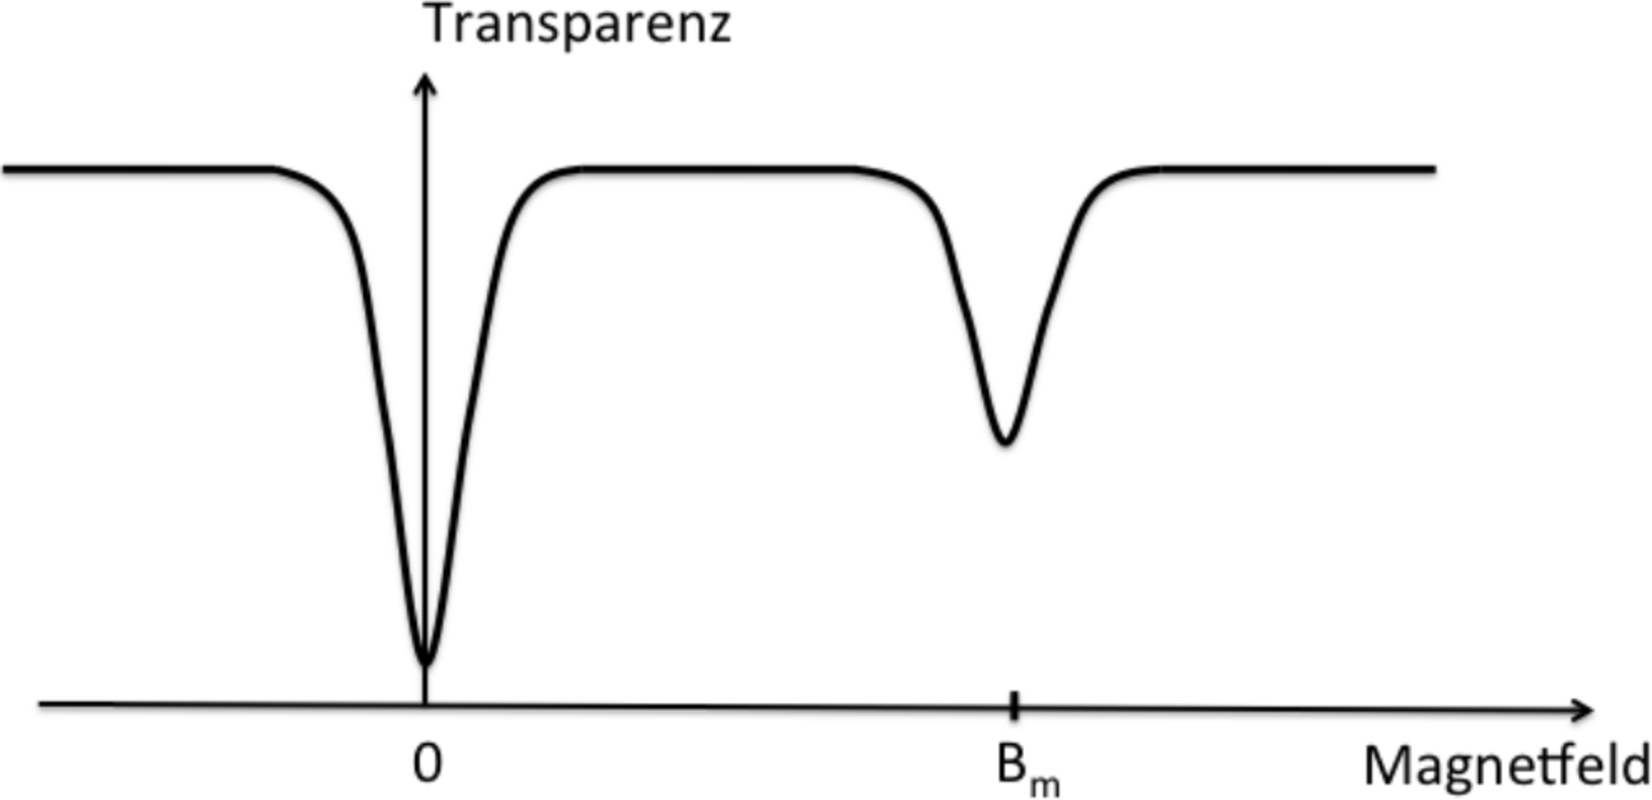
\includegraphics[width=0.6\textwidth]{transparenzkurve.pdf}
  \caption{Verlauf der Transparenz der Dampfzelle in Abhängigkeit des äußeren Magnetfeldes \cite{anleitung}.}
  \label{fig:transparenz_b}
\end{figure}
%


\subsection{Der quadratische Zeeman-Effekt}

Die Aufspaltung der Zeeman-Niveaus verhält sich allerdings nicht für alle Magnetfeldstärken
wie in Abbildung~\ref{fig:aufspaltung} dargestellt. Für große Magnetfelder werden höhere
Ordnungen in Abhängigkeit des Magnetfeldes relevant, sodass die Zeeman-Aufspaltung durch
%
\begin{equation}
  \mathup{U}_\mathup{HF} = g_{\mathup{F}}\mu_{\mathup{B}}B + g_{\mathup{F}}^2\mu_{\mathup{B}}^2B^2\frac{(1-2M_\mathup{F})}{\symup{\Delta} \mathup{E_{Hy}}} - ....
  \label{eq:quad_zeeman}
\end{equation}
%
beschrieben wird. Dabei ist $\symup{\Delta} \mathup{E_{Hy}}$ die Energiedifferenz der
Hyperfeinstrukturaufspaltung zwischen den Niveaus $\mathup{F}$ und $\mathup{F}+1$.
Hier werden nun neben den Wechselwirkungen der magnetischen Momente mit dem äußeren
Magnetfeld auch diese zwischen den magnetischen Momenten berücksichtigt.

\section{Durchführung}
\label{sec:durchführung}

\subsection{Der Versuchsaufbau}
Abbildung~\ref{fig:aufbau} zeigt den schematischen Aufbau der Versuchsapparatur.
Ausgangspunkt des untersuchten Lichtes ist eine Spektrallampe. Dabei handelt es
sich um eine Rubidiumdampflampe. Das Licht dieser Lampe wird über eine
Sammellinse fokussiert und parallelisiert. Ein D1-Filter selektiert aus diesem
Licht ein schmales Frequenzspektrum heraus. Dabei handelt es sich um die
D1-Linie des Rubidiums, welche eine Wellenlänge von etwa
$\lambda=\SI{794.8}{\nano\metre}$ besitzt. Der Filter stellt ein von einer
refĺektierenden Schicht umgebenes Dielektrikum der Dicke $d$ und
Brechungsindex $n$ dar. Die äußere Schicht ist für Licht halbdurchlässig,
weswegen einfallendes Licht innerhalb des Dielektrikums mehrfach reflektiert
wird. Dies führt dazu, dass Wellenlängen der Größe
%
\begin{equation}
  m\cdot\lambda_m=2\cdot n\cdot d+\frac{\lambda}{2}, \quad m=2,3,\ldots
\end{equation}
%
konstruktiv interferieren. Licht einer anderen Wellenlänge hingegen wird so
durch destruktive Interferenz herausgefiltert. Durch einen Polarisationsfilter
wird das Licht anschließend linear polarisiert, um anschließend durch ein
$\sfrac{\lambda}{4}$-Plättchen zirkular polarisiert zu werden. Das
$\sfrac{\lambda}{4}$-Plättchen stellt eine aus einem anisotropen Material
besthende Verzögerungsvorrichtung dar. Sie ist in der Lage einfallendes Licht
entlang zweier Achsen unterschiedlich zu verzögern, sodass durch die Ausrichtung
der gewünschte Phasenunterschied zwischen einzelnen Komponenten des Lichtes
erzeugt werden kann. Für zirkular polarisiertes Licht aus linear polarisiertem Licht,
muss diese Ausrichtung gerade einen Winkel von $\sfrac{\pi}{2}$ betragen. \\
Das nun hinreichend präparierte Licht fällt anschließend auf eine Dampfzelle.
Diese ist mit Rubidiumgas gefüllt und elektrisch beheizbar. Die Temperaturerhöhung
sorgt dafür, dass die thermische Verteilung der Energie breiter ist, sowie zur
Regulierung des Dampfdruckes innerhalb der Zelle. Die Zelle befindet sich
innerhalb mehrerer Helmholtzspulenpaare. Ein Paar ist horizontal ausgerichtet
(Horizontalfeldspule), während das zweite Paar vertikal ausgerichtet ist. Dazu
geschaltet ist eine Modulationsfeldspule (Sweep-Spule). Alle Spulen lassen sich
einzeln über die Feldströme steuern. Zusätzlich zu den Helmholtzspulen besitzt
die Apparatur auch eine RF-Spule. Mit dieser lassen sich elektromagnetische Wellen
bestimmter Frequenz erzeugen, die für die induzierte Emission verwendet werden.
Nachdem das Licht die Dampfzellle passiert hat wird es durch eine Sammellinse
wieder fokussiert und anschließend von einem Lichtdetektor vermessen.
Dazu wird ein Si-Photoelement verwendet, welches das Licht in ein elektrisches
Signal wandelt. Dieses wird durch ein Oszilloskop eingelesen und dargestellt.
Zur Abschirmung von Außenlicht wird der gesamte Messaufbau während der Messung
mit einer schwarzen Stoffdecke abgedunkelt.

\subsection{Die Versuchsdurchführung}
Da es sich hierbei um einen optischen Aufbau mit mehreren optischen Elementen
handelt, muss die Apperatur zunächst so eingestellt werden, dass das vermessene
Licht eine maximale Intensität aufweist. Dazu wird der Polarisationsfilter
sowie das $\sfrac{\lambda}{4}$-Plättchen zunächst aus dem Strahlengang entfernt.
Da die Magnetfeldstärken der verwendeten Spulen in der Größenordnung des
Erdmagnetfeldes liegen, muss dieses möglichst kompensiert werden. Dazu wird der
gesamte Versuchsaufbau entlang der optischen Achse in Nord-Süd-Richtung
ausgerichtet. Dies dient zur Kompensation der horizontalen Komponente des
Magnetfeldes. Die vertikale Komponente wird durch die Vertikalspule
ausgeglichen. Dazu wird der Spulenstrom solange variiert, bis der auf dem
Oszilloskop dargestellte Bereich des Transparenzminimums eine minimale Breite aufweist.
Zur Verringerung des Einflusses äußeren Lichtes wird der Aufbau nun durch eine
schwarze Stoffdecke abgeschirmt.
\clearpage
\noindent
Zur Vermessung der Zeeman-Aufspaltung wird über die RF-Spule stufenweise ein äußeres
hochfrequentes Magnetfeld angelegt ($\SI{100}{\kilo\hertz}$ bis $\SI{1}{\mega\hertz}$).
Dieses wird über eine Sinusspannung an einem HF-Generator erzeugt. Ziel ist es, die in
Abbildung~\ref{fig:transparenz_b} dargestellten \enquote{dips} auf dem Oszilloskop
zu untersuchen. Dazu werden für jede Frequenz die Spulenströme von Horizontalfeld-
und Sweepspule bei den \enquote{dips} abgelesen.\\

\end{document}
